
% !TEX TS-program = lualatex
\documentclass[11pt]{article}

\usepackage[margin=1in]{geometry}
\usepackage{lmodern} % Latin Modern fonts (works with LuaLaTeX)
\usepackage{microtype}
\usepackage{amsmath,amssymb}
\usepackage{hyperref}
\usepackage{tikz}
\usetikzlibrary{calc,angles,quotes,intersections,decorations.markings,through}


\hypersetup{
  colorlinks=true,
  linkcolor=blue,
  urlcolor=blue
}

% --- TikZ helpers (ticks + right-angle marks) ---
\tikzset{
  tick/.style={
    postaction={decorate},
    decoration={markings,
      mark=at position 0.5 with {\draw (-2pt,-2pt)--(2pt,2pt);}
    }
  },
  tick2/.style={
    postaction={decorate},
    decoration={markings,
      mark=at position 0.45 with {\draw (-2pt,-2pt)--(2pt,2pt);},
      mark=at position 0.55 with {\draw (-2pt,-2pt)--(2pt,2pt);}
    }
  },
  tick3/.style={
    postaction={decorate},
    decoration={markings,
      mark=at position 0.43 with {\draw (-2pt,-2pt)--(2pt,2pt);},
      mark=at position 0.50 with {\draw (-2pt,-2pt)--(2pt,2pt);},
      mark=at position 0.57 with {\draw (-2pt,-2pt)--(2pt,2pt);}
    }
  }
}

\newcommand{\theoremblock}[3]{%
  \subsection*{#1}%
  \textbf{Theorem.} #2\par
  \textbf{Suggested abbreviation.} #3\par
}

\newcommand{\diagram}{\par\medskip\noindent\textbf{Diagram.}\par\smallskip}

\title{Circle geometry theorems}
\author{}
\date{}

\begin{document}
\maketitle

\noindent\textbf{Source:}
\href{http://topdrawer.aamt.edu.au/Geometric-reasoning/Big-ideas/Circle-geometry/Angle-and-chord-properties}{http://topdrawer.aamt.edu.au/Geometric-reasoning/Big-ideas/Circle-geometry/Angle-and-chord-properties}

\section*{Circle geometry theorems}

\theoremblock{1. Intersecting circles: centres bisect common chord}{When two circles intersect, the line joining their centres bisects their common chord at right angles.}{centres of touching circles}
\diagram
\begin{center}
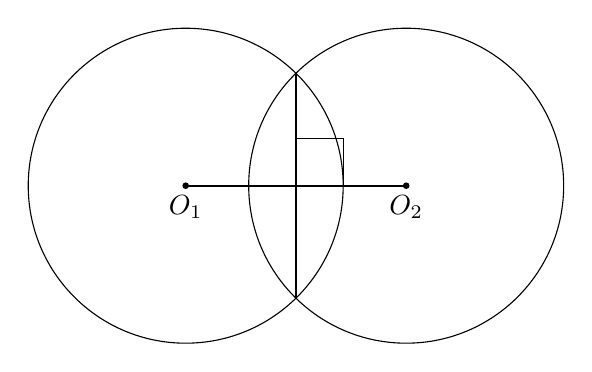
\begin{tikzpicture}[scale=1]
  \def\R{2.0}
  \coordinate (O1) at (-1.4,0);
  \coordinate (O2) at ( 1.4,0);
  % Two equal circles
  \draw (O1) circle (\R);
  \draw (O2) circle (\R);

  % Intersection points (computed for r=2, d=2.8 -> x=0, y=sqrt(r^2-(d/2)^2))
  \coordinate (I1) at (0, 1.428);
  \coordinate (I2) at (0,-1.428);

  % Common chord
  \draw[thick] (I1) -- (I2);
  % Line of centres
  \draw[thick] (O1) -- (O2);
  % Right angle at intersection of chord and centres line (origin)
  \coordinate (M) at (0,0);
  \pic[draw, angle radius=6mm] {right angle = I1--M--O2};

  \fill (O1) circle (1.2pt) node[below] {$O_1$};
  \fill (O2) circle (1.2pt) node[below] {$O_2$};
\end{tikzpicture}
\end{center}

\theoremblock{2. Equal arcs in equal circles $\Leftrightarrow$ equal central angles}{Equal arcs on circles of equal radii subtend equal angles at the centre, and conversely.}{equal arcs, equal angles}
\diagram
\begin{center}
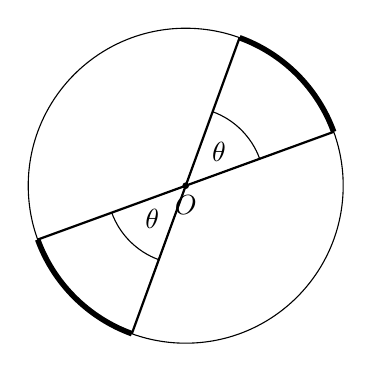
\begin{tikzpicture}[scale=1]
  \def\R{2.0}
  \coordinate (O) at (0,0);
  \draw (O) circle (\R);

  % Two equal arcs (shown bold) with equal central angles
  \coordinate (A) at (70:\R);
  \coordinate (B) at (20:\R);
  \coordinate (C) at (-110:\R);
  \coordinate (D) at (-160:\R);

  \draw[thick] (O) -- (A) (O) -- (B);
  \draw[thick] (O) -- (C) (O) -- (D);

  % Highlight arcs AB and CD
  \draw[line width=2pt] (A) arc[start angle=70,end angle=20,radius=\R];
  \draw[line width=2pt] (C) arc[start angle=-110,end angle=-160,radius=\R];

  \fill (O) circle(1.2pt) node[below] {$O$};

  \pic[draw, "$\theta$", angle radius=10mm] {angle = B--O--A};
  \pic[draw, "$\theta$", angle radius=10mm] {angle = D--O--C};
\end{tikzpicture}
\end{center}

\theoremblock{3. Equal central angles $\Leftrightarrow$ equal chords}{Equal angles at the centre stand on equal chords, and conversely.}{equal chords, equal angles \quad OR \quad angles standing on equal chords \quad OR \quad angles standing on equal arcs}
\diagram
\begin{center}
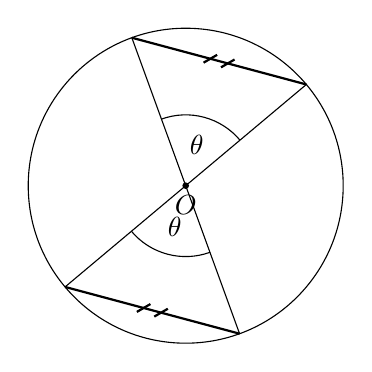
\begin{tikzpicture}[scale=1]
  \def\R{2.0}
  \coordinate (O) at (0,0);
  \draw (O) circle (\R);

  \coordinate (A) at (110:\R);
  \coordinate (B) at (40:\R);
  \coordinate (C) at (-70:\R);
  \coordinate (D) at (-140:\R);

  % Chords
  \draw[thick,tick2] (A) -- (B);
  \draw[thick,tick2] (C) -- (D);

  % Radii for angles
  \draw (O) -- (A) (O) -- (B);
  \draw (O) -- (C) (O) -- (D);

  \fill (O) circle(1.2pt) node[below] {$O$};

  \pic[draw, "$\theta$", angle radius=9mm] {angle = B--O--A};
  \pic[draw, "$\theta$", angle radius=9mm] {angle = D--O--C};
\end{tikzpicture}
\end{center}

\bigskip

\theoremblock{4. Central angle is twice circumferential angle}{The angle at the centre is twice the angle at the circumference subtended by the same arc.}{angles at the centre and circumference}
\diagram
\begin{center}
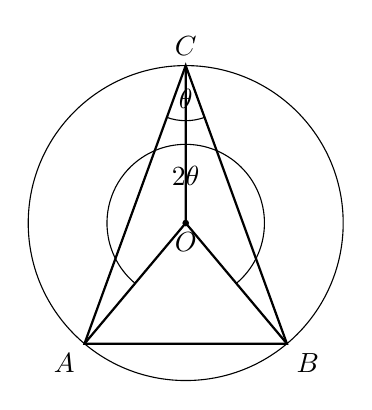
\begin{tikzpicture}[scale=1]
  \def\R{2.0}
  \coordinate (O) at (0,0);
  \draw (O) circle (\R);

  \coordinate (A) at (230:\R);
  \coordinate (B) at (-50:\R);
  \coordinate (C) at (90:\R);

  \draw[thick] (A) -- (C) -- (B) -- cycle;
  \draw[thick] (O) -- (A) (O) -- (B) (O) -- (C);

  \fill (O) circle(1.2pt) node[below] {$O$};
  \node[below left] at (A) {$A$};
  \node[below right] at (B) {$B$};
  \node[above] at (C) {$C$};

  \pic[draw, "$\theta$", angle radius=7mm] {angle = A--C--B};
  \pic[draw, "$2\theta$", angle radius=10mm] {angle = B--O--A};
\end{tikzpicture}
\end{center}

\theoremblock{5. Tangent $\perp$ radius at point of contact}{The tangent to a circle is perpendicular to the radius drawn to the point of contact and conversely.}{tangent perpendicular to radius}
\diagram
\begin{center}
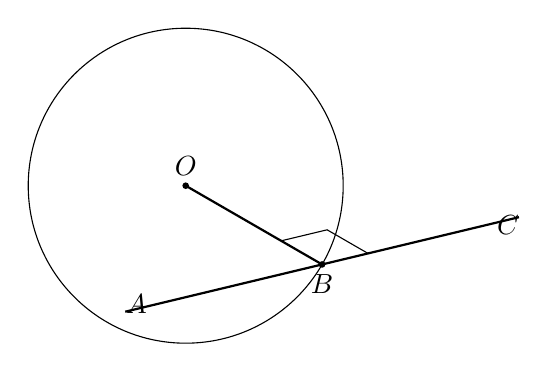
\begin{tikzpicture}[scale=1]
  \def\R{2.0}
  \coordinate (O) at (0,0);
  \draw (O) circle (\R);

  \coordinate (B) at (-30:\R);
  % Tangent line at B
  \draw[thick] ($(B)+(-2.5,-0.6)$) -- ($(B)+(2.5,0.6)$);
  \draw[thick] (O) -- (B);

  \coordinate (Tg) at ($(B)+(2.5,0.6)$);
  \pic[draw, angle radius=6mm] {right angle = O--B--Tg};

  \fill (O) circle(1.2pt) node[above] {$O$};
  \fill (B) circle(1.2pt) node[below] {$B$};
  \node[left] at ($(B)+(-2.1,-0.5)$) {$A$};
  \node[right] at ($(B)+(2.1,0.5)$) {$C$};
\end{tikzpicture}
\end{center}

\theoremblock{6. Perpendicular from centre to chord bisects chord}{The perpendicular from the centre of a circle to a chord bisects the chord.}{perpendicular from the centre}
\diagram
\begin{center}
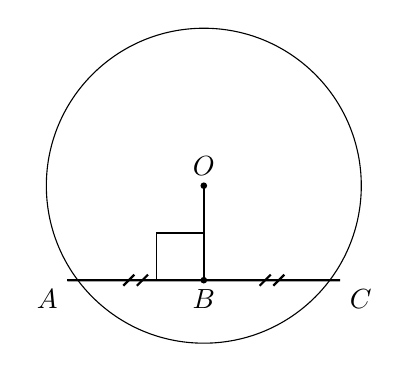
\begin{tikzpicture}[scale=1]
  \def\R{2.0}
  \coordinate (O) at (0,0.2);
  \draw (O) circle (\R);

  \coordinate (A) at (210:\R);
  \coordinate (C) at (-30:\R);
  \coordinate (B) at ($(A)!0.5!(C)$);

  \draw[thick] (A) -- (C);
  \draw[thick] (O) -- (B);

  % Mark equal halves of chord
  \draw[thick,tick2] (A) -- (B);
  \draw[thick,tick2] (B) -- (C);

  \pic[draw, angle radius=6mm] {right angle = A--B--O};

  \fill (O) circle(1.2pt) node[above] {$O$};
  \node[below left] at (A) {$A$};
  \node[below right] at (C) {$C$};
  \fill (B) circle(1.2pt) node[below] {$B$};
\end{tikzpicture}
\end{center}

\theoremblock{7. Centre to midpoint of chord is perpendicular to chord}{The line from the centre of a circle to the midpoint of a chord is perpendicular to the chord.}{line joining centre to midpoint of chord}
\diagram
\begin{center}
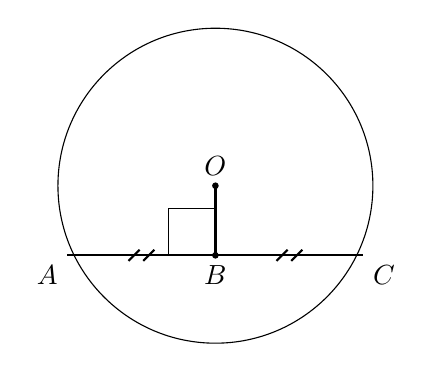
\begin{tikzpicture}[scale=1]
  \def\R{2.0}
  \coordinate (O) at (0,0.2);
  \draw (O) circle (\R);

  \coordinate (A) at (200:\R);
  \coordinate (C) at (-20:\R);
  \coordinate (B) at ($(A)!0.5!(C)$);

  \draw[thick] (A) -- (C);
  \draw[thick] (O) -- (B);

  \draw[thick,tick2] (A) -- (B);
  \draw[thick,tick2] (B) -- (C);

  \pic[draw, angle radius=6mm] {right angle = A--B--O};

  \fill (O) circle(1.2pt) node[above] {$O$};
  \node[below left] at (A) {$A$};
  \node[below right] at (C) {$C$};
  \fill (B) circle(1.2pt) node[below] {$B$};
\end{tikzpicture}
\end{center}

\theoremblock{8. Perpendicular bisector of a chord passes through centre}{The perpendicular bisector of a chord passes through the centre of the circle.}{perpendicular bisector of chord}
\diagram
\begin{center}
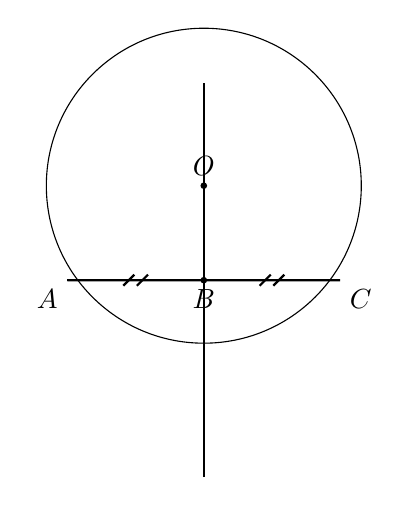
\begin{tikzpicture}[scale=1]
  \def\R{2.0}
  \coordinate (O) at (0,0.2);
  \draw (O) circle (\R);

  \coordinate (A) at (210:\R);
  \coordinate (C) at (-30:\R);
  \coordinate (B) at ($(A)!0.5!(C)$);

  \draw[thick] (A) -- (C);
  % Perpendicular bisector line
  \draw[thick] ($(B)+(0,-2.5)$) -- ($(B)+(0,2.5)$);
  \draw[thick,tick2] (A) -- (B);
  \draw[thick,tick2] (B) -- (C);

  \fill (O) circle(1.2pt) node[above] {$O$};
  \node[below left] at (A) {$A$};
  \node[below right] at (C) {$C$};
  \fill (B) circle(1.2pt) node[below] {$B$};
\end{tikzpicture}
\end{center}

\bigskip

\theoremblock{9. Equal chords in equal circles are equidistant from centre}{Equal chords in equal circles are equidistant from the centres.}{equal chords equidistant from centre}
\diagram
\begin{center}
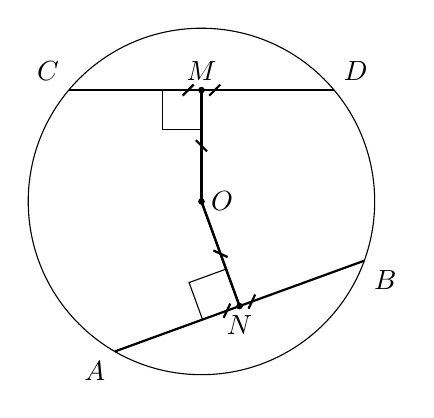
\begin{tikzpicture}[scale=1]
  \def\R{2.2}
  \coordinate (O) at (0,0);
  \draw (O) circle (\R);

  % Two equal chords (top and lower-right)
  \coordinate (C) at (140:\R);
  \coordinate (D) at (40:\R);
  \coordinate (A) at (-120:\R);
  \coordinate (B) at (-20:\R);

  \coordinate (M) at ($(C)!0.5!(D)$);
  \coordinate (N) at ($(A)!0.5!(B)$);

  \draw[thick,tick2] (C) -- (D);
  \draw[thick,tick2] (A) -- (B);

  \draw[thick] (O) -- (M);
  \draw[thick] (O) -- (N);

  \pic[draw, angle radius=5mm] {right angle = C--M--O};
  \pic[draw, angle radius=5mm] {right angle = A--N--O};

  % Mark equal distances OM and ON (two ticks)
  \draw[thick,tick] (O) -- (M);
  \draw[thick,tick] (O) -- (N);

  \fill (O) circle(1.2pt) node[right] {$O$};
  \node[above left] at (C) {$C$};
  \node[above right] at (D) {$D$};
  \node[below left] at (A) {$A$};
  \node[below right] at (B) {$B$};
  \fill (M) circle(1.2pt) node[above] {$M$};
  \fill (N) circle(1.2pt) node[below] {$N$};
\end{tikzpicture}
\end{center}

\theoremblock{10. Chords equidistant from centre are equal}{Chords in a circle which are equidistant from the centre are equal.}{equal chords equidistant from centre}
\diagram
\begin{center}
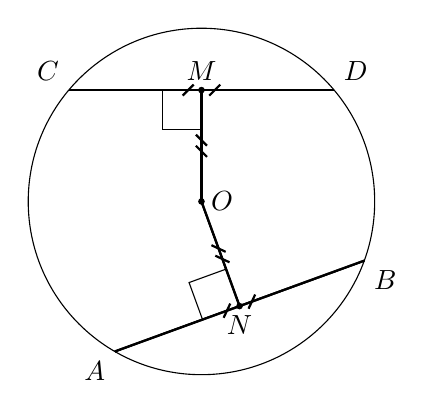
\begin{tikzpicture}[scale=1]
  \def\R{2.2}
  \coordinate (O) at (0,0);
  \draw (O) circle (\R);

  \coordinate (C) at (140:\R);
  \coordinate (D) at (40:\R);
  \coordinate (A) at (-120:\R);
  \coordinate (B) at (-20:\R);

  \coordinate (M) at ($(C)!0.5!(D)$);
  \coordinate (N) at ($(A)!0.5!(B)$);

  % Equal distances from centre (ticks on OM and ON)
  \draw[thick,tick2] (O) -- (M);
  \draw[thick,tick2] (O) -- (N);

  \draw[thick] (C) -- (D);
  \draw[thick] (A) -- (B);
  \draw[thick] (O) -- (M);
  \draw[thick] (O) -- (N);

  \pic[draw, angle radius=5mm] {right angle = C--M--O};
  \pic[draw, angle radius=5mm] {right angle = A--N--O};

  % Mark chords equal (double ticks)
  \draw[thick,tick2] (C) -- (D);
  \draw[thick,tick2] (A) -- (B);

  \fill (O) circle(1.2pt) node[right] {$O$};
  \node[above left] at (C) {$C$};
  \node[above right] at (D) {$D$};
  \node[below left] at (A) {$A$};
  \node[below right] at (B) {$B$};
  \fill (M) circle(1.2pt) node[above] {$M$};
  \fill (N) circle(1.2pt) node[below] {$N$};
\end{tikzpicture}
\end{center}

\theoremblock{11. Three non-collinear points determine a unique circle (circumcentre)}{Any three non-collinear points lie on a unique circle, whose centre is the point of concurrency of the perpendicular bisectors of the intervals joining the points.}{perpendicular bisector of chord passes through the centre}
\diagram
\begin{center}
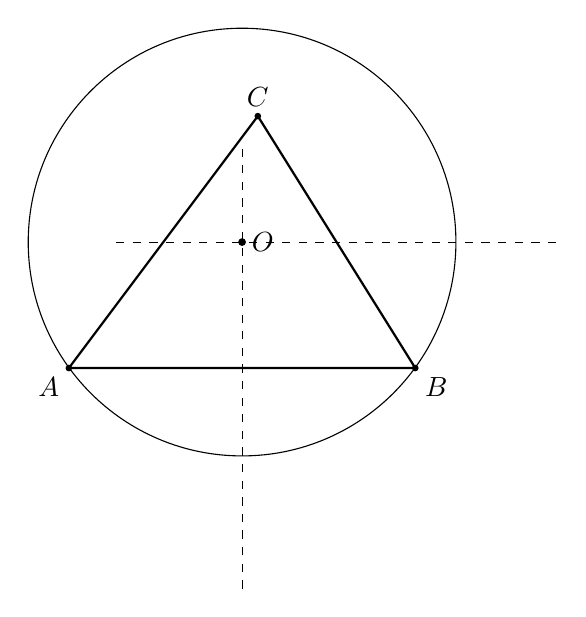
\begin{tikzpicture}[scale=1]
  \coordinate (A) at (-2.2,-1.0);
  \coordinate (B) at ( 2.2,-1.0);
  \coordinate (C) at ( 0.2, 2.2);

  % Circumcircle
  \path[name path=AB] (A) -- (B);
  \path[name path=BC] (B) -- (C);
  \path[name path=CA] (C) -- (A);

  % Compute circumcenter using perpendicular bisectors intersections
  \coordinate (Mab) at ($(A)!0.5!(B)$);
  \coordinate (Mbc) at ($(B)!0.5!(C)$);

  \path[name path=pbAB] (Mab) -- ($(Mab)+(0,3)$);
  \path[name path=pbBC] (Mbc) -- ($(Mbc)+(-3,0)$);

  % Choose explicit perpendicular bisectors for drawing (dashed)
  \draw[dashed] ($(Mab)+(-0.0,-2.8)$) -- ($(Mab)+(0.0,2.8)$);
  \draw[dashed] ($(Mbc)+(-2.8,0.0)$) -- ($(Mbc)+(2.8,0.0)$);

  % Circumcenter (computed by TikZ calc: use intersection of the two dashed lines)
  \path[name path=V1] ($(Mab)+(-0.0,-2.8)$) -- ($(Mab)+(0.0,2.8)$);
  \path[name path=V2] ($(Mbc)+(-2.8,0.0)$) -- ($(Mbc)+(2.8,0.0)$);
  \path [name intersections={of=V1 and V2, by=O}];

  % Draw circumcircle through A (centre O)
  \node[draw, circle through={(A)}] at (O) {};

  % Triangle
  \draw[thick] (A) -- (B) -- (C) -- cycle;

  \fill (O) circle (1.4pt) node[right] {$O$};
  \fill (A) circle (1.2pt) node[below left] {$A$};
  \fill (B) circle (1.2pt) node[below right] {$B$};
  \fill (C) circle (1.2pt) node[above] {$C$};
\end{tikzpicture}
\end{center}

\theoremblock{12. Angles in the same segment are equal}{Angles in the same segment are equal.}{angles in the same segment}
\diagram
\begin{center}
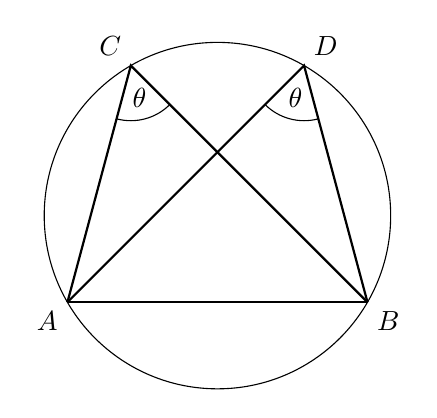
\begin{tikzpicture}[scale=1]
  \def\R{2.2}
  \coordinate (O) at (0,0);
  \draw (O) circle (\R);

  \coordinate (A) at (210:\R);
  \coordinate (B) at (-30:\R);
  \coordinate (C) at (120:\R);
  \coordinate (D) at (60:\R);

  \draw[thick] (A) -- (B);
  \draw[thick] (A) -- (C) -- (B);
  \draw[thick] (A) -- (D) -- (B);

  \pic[draw, "$\theta$", angle radius=7mm] {angle = A--C--B};
  \pic[draw, "$\theta$", angle radius=7mm] {angle = A--D--B};

  \node[below left] at (A) {$A$};
  \node[below right] at (B) {$B$};
  \node[above left] at (C) {$C$};
  \node[above right] at (D) {$D$};
\end{tikzpicture}
\end{center}

\theoremblock{13. Angle in a semi-circle is a right angle}{The angle in a semi-circle is a right angle.}{angle in a semi-circle}
\diagram
\begin{center}
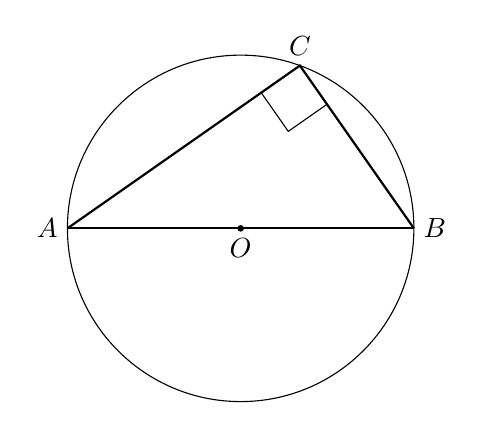
\begin{tikzpicture}[scale=1]
  \def\R{2.2}
  \coordinate (O) at (0,0);
  \draw (O) circle (\R);

  \coordinate (A) at (180:\R);
  \coordinate (B) at (0:\R);
  \coordinate (C) at (70:\R);

  \draw[thick] (A) -- (B); % diameter
  \draw[thick] (A) -- (C) -- (B);

  \pic[draw, angle radius=6mm] {right angle = A--C--B};

  \fill (O) circle(1.2pt) node[below] {$O$};
  \node[left] at (A) {$A$};
  \node[right] at (B) {$B$};
  \node[above] at (C) {$C$};
\end{tikzpicture}
\end{center}

\bigskip

\theoremblock{14. Opposite angles of a cyclic quadrilateral are supplementary}{Opposite angles of a cyclic quadrilateral are supplementary.}{opposite angles in a cyclic quad \quad $x+y=180$}
\diagram
\begin{center}
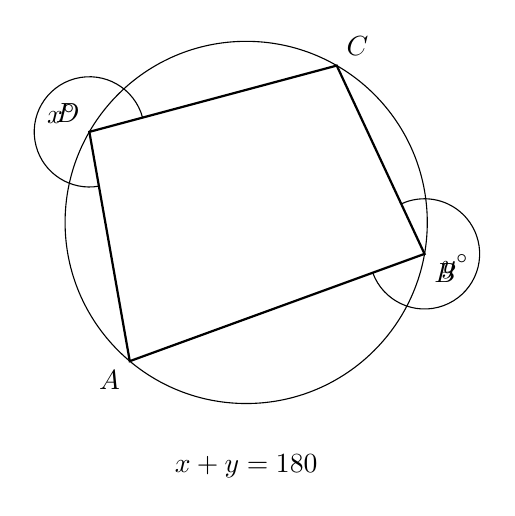
\begin{tikzpicture}[scale=1]
  \def\R{2.3}
  \coordinate (O) at (0,0);
  \draw (O) circle (\R);

  \coordinate (A) at (230:\R);
  \coordinate (B) at (-10:\R);
  \coordinate (C) at (60:\R);
  \coordinate (D) at (150:\R);

  \draw[thick] (A) -- (B) -- (C) -- (D) -- cycle;

  \pic[draw, "$x^\circ$", angle radius=7mm] {angle = C--D--A};
  \pic[draw, "$y^\circ$", angle radius=7mm] {angle = A--B--C};

  \node[below left] at (A) {$A$};
  \node[below right] at (B) {$B$};
  \node[above right] at (C) {$C$};
  \node[above left] at (D) {$D$};

  \node at (0,-3.1) {$x+y=180$};
\end{tikzpicture}
\end{center}

\theoremblock{15. Exterior angle of a cyclic quadrilateral}{The exterior angle at a vertex of a cyclic quadrilateral is equal to the interior opposite angle.}{exterior angle of cyclic quad}
\diagram
\begin{center}
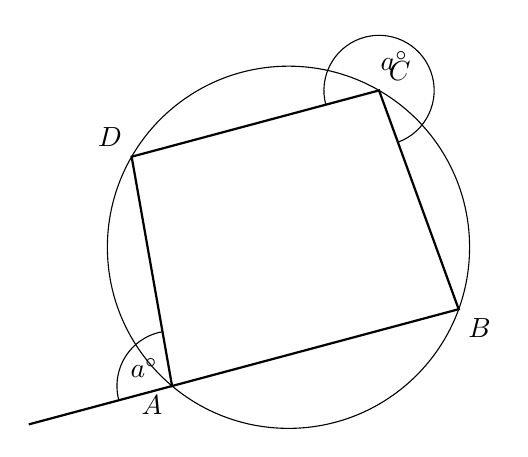
\begin{tikzpicture}[scale=1]
  \def\R{2.3}
  \coordinate (O) at (0,0);
  \draw (O) circle (\R);

  \coordinate (A) at (230:\R);
  \coordinate (B) at (-20:\R);
  \coordinate (C) at (60:\R);
  \coordinate (D) at (150:\R);

  \draw[thick] (A) -- (B) -- (C) -- (D) -- cycle;

  % Extend AB beyond A to create exterior angle at A
  \coordinate (E) at ($(A)!-0.5!(B)$);
  \draw[thick] (A) -- (E);

  \pic[draw, "$a^\circ$", angle radius=7mm] {angle = D--A--E}; % exterior at A
  \pic[draw, "$a^\circ$", angle radius=7mm] {angle = B--C--D}; % interior opposite at C

  \node[below left] at (A) {$A$};
  \node[below right] at (B) {$B$};
  \node[above right] at (C) {$C$};
  \node[above left] at (D) {$D$};
\end{tikzpicture}
\end{center}

\theoremblock{16. Converse: supplementary opposite angles $\Rightarrow$ cyclic}{If the opposite angles in a quadrilateral are supplementary then the quadrilateral is cyclic.\\\emph{Note: This theorem is also a test for four points to be concyclic.}}{converse of opposite angles in a cyclic quad \quad If $x+y=180$ then $ABCD$ is a cyclic quadrilateral.}
\diagram
\begin{center}
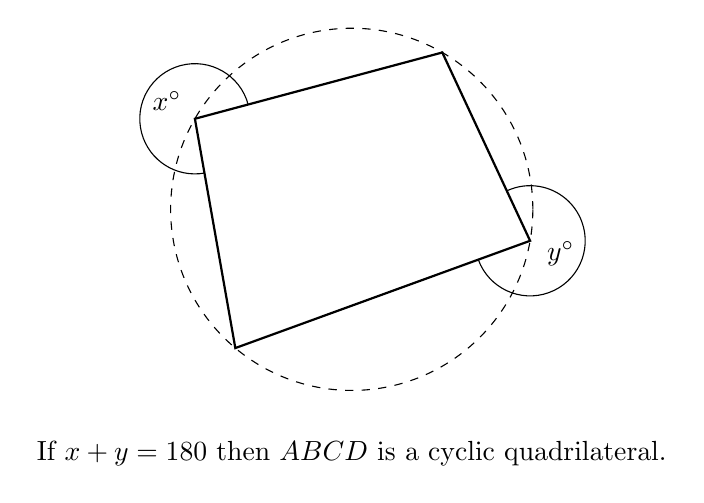
\begin{tikzpicture}[scale=1]
  \def\R{2.3}
  \coordinate (O) at (0,0);
  \draw[dashed] (O) circle (\R);

  \coordinate (A) at (230:\R);
  \coordinate (B) at (-10:\R);
  \coordinate (C) at (60:\R);
  \coordinate (D) at (150:\R);

  \draw[thick] (A) -- (B) -- (C) -- (D) -- cycle;

  \pic[draw, "$x^\circ$", angle radius=7mm] {angle = C--D--A};
  \pic[draw, "$y^\circ$", angle radius=7mm] {angle = A--B--C};

  \node at (0,-3.1) {If $x+y=180$ then $ABCD$ is a cyclic quadrilateral.};
\end{tikzpicture}
\end{center}

\theoremblock{17. Intersecting chords (power of a point)}{The products of the intercepts of two intersecting chords are equal.}{intersecting chords \quad $AP\times BP = CP\times DP$}
\diagram
\begin{center}
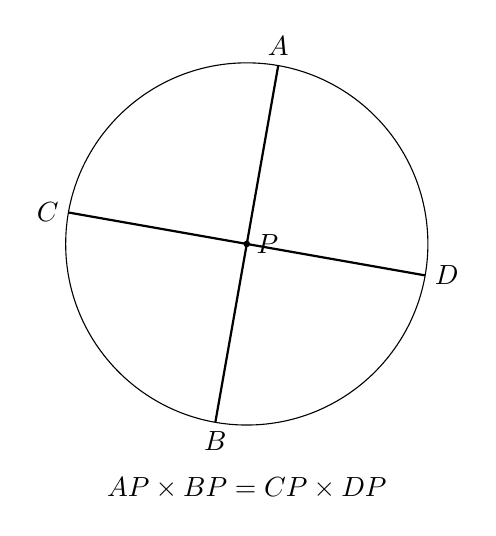
\begin{tikzpicture}[scale=1]
  \def\R{2.3}
  \coordinate (O) at (0,0);
  \draw (O) circle (\R);

  \coordinate (A) at (80:\R);
  \coordinate (B) at (-100:\R);
  \coordinate (C) at (170:\R);
  \coordinate (D) at (-10:\R);

  \path [name path=ch1] (A) -- (B);
  \path [name path=ch2] (C) -- (D);
  \path [name intersections={of=ch1 and ch2, by=P}];

  \draw[thick] (A) -- (B);
  \draw[thick] (C) -- (D);

  \fill (P) circle(1.2pt) node[right] {$P$};
  \node[above] at (A) {$A$};
  \node[below] at (B) {$B$};
  \node[left] at (C) {$C$};
  \node[right] at (D) {$D$};

  \node at (0,-3.1) {$AP\times BP = CP\times DP$};
\end{tikzpicture}
\end{center}

\bigskip

\theoremblock{18. Intersecting secants from an external point}{The products of the intercepts of two intersecting secants to a circle from an external point.}{intersecting secants \quad $AP\times BP = CP\times DP$}
\diagram
\begin{center}
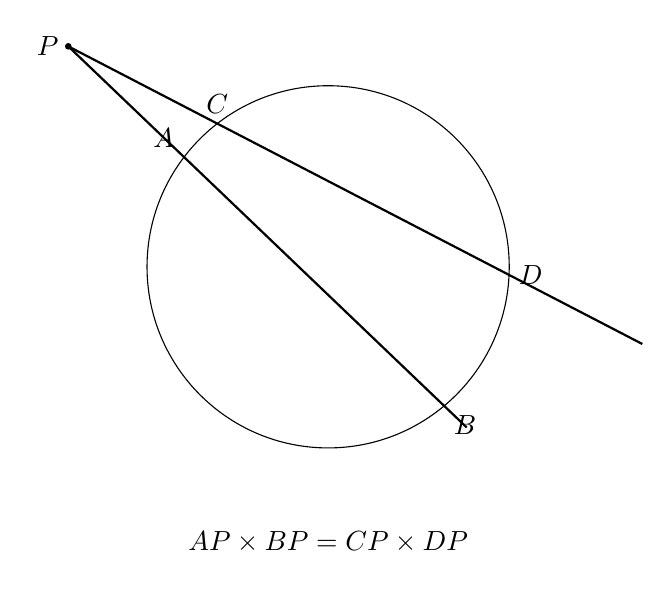
\begin{tikzpicture}[scale=1]
  \def\R{2.3}
  \coordinate (O) at (0,0);
  \draw (O) circle (\R);

  \coordinate (P) at (-3.3, 2.8);

  % Two secants from P
  \coordinate (dir1) at (-1.0,0.6);
  \coordinate (s1b) at ($(P)!2.2!(dir1)$); % extend beyond the circle
  \draw[thick] (P) -- (s1b);

  \coordinate (dir2) at (-0.6,1.4);
  \coordinate (s2b) at ($(P)!2.7!(dir2)$); % extend beyond the circle
  \draw[thick] (P) -- (s2b);

  % Find intersections with circle for labeling
  \path[name path=circle] (O) circle (\R);
  \path[name path=sec1] (P) -- (s1b);
  \path[name path=sec2] (P) -- (s2b);

  \path[name intersections={of=circle and sec1, by={A,B}}];
  \path[name intersections={of=circle and sec2, by={C,D}}];

  \fill (P) circle(1.2pt) node[left] {$P$};
  \node[above left] at (A) {$A$};
  \node[below right] at (B) {$B$};
  \node[above] at (C) {$C$};
  \node[right] at (D) {$D$};

  \node at (0,-3.5) {$AP\times BP = CP\times DP$};
\end{tikzpicture}
\end{center}

\theoremblock{19. Tangents from an external point are equal}{Tangents to a circle from an external point are equal.}{tangents from external point}
\diagram
\begin{center}
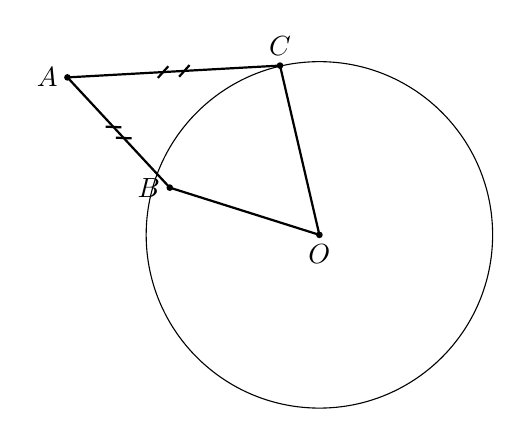
\begin{tikzpicture}[scale=1]
  \def\R{2.2}
  \coordinate (O) at (0,0);
  \draw (O) circle (\R);

  \coordinate (A) at (-3.2, 2.0);

  % Construct tangency points roughly
  \coordinate (B) at (-1.9, 0.6);
  \coordinate (C) at (-0.5, 2.15);

  \draw[thick,tick2] (A) -- (B);
  \draw[thick,tick2] (A) -- (C);

  \draw[thick] (O) -- (B);
  \draw[thick] (O) -- (C);

  \fill (O) circle(1.2pt) node[below] {$O$};
  \fill (A) circle(1.2pt) node[left] {$A$};
  \fill (B) circle(1.2pt) node[left] {$B$};
  \fill (C) circle(1.2pt) node[above] {$C$};
\end{tikzpicture}
\end{center}

\theoremblock{20. Alternate segment theorem (tangent--chord angle)}{The angle between a tangent and a chord through the point of contact is equal to the angle in the alternate segment.}{angle in alternate segment \quad OR \quad angle between tangent and chord}
\diagram
\begin{center}
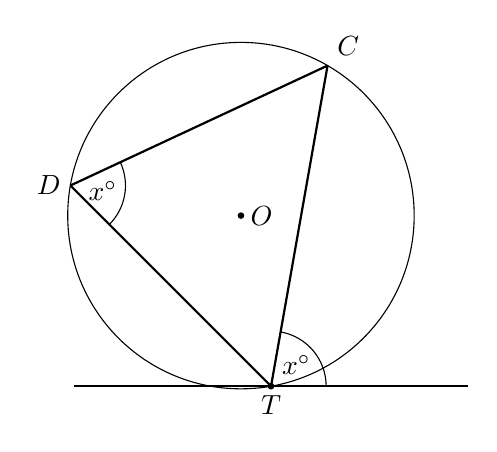
\begin{tikzpicture}[scale=1]
  \def\R{2.2}
  \coordinate (O) at (0,0);
  \draw (O) circle (\R);

  \coordinate (T) at (-80:\R); % point of tangency
  \coordinate (C) at (60:\R);  % chord endpoint
  \coordinate (D) at (170:\R); % alternate segment point

  % Tangent at T (approx direction)
  \draw[thick] ($(T)+(-2.5,0)$) -- ($(T)+(2.5,0)$);

  % Chord through T to C
  \draw[thick] (T) -- (C);

  % Angle in alternate segment at D
  \draw[thick] (D) -- (T);
  \draw[thick] (D) -- (C);

  \coordinate (Tdir) at ($(T)+(2.5,0)$);
  \pic[draw, "$x^\circ$", angle radius=7mm] {angle = Tdir--T--C};
  \pic[draw, "$x^\circ$", angle radius=7mm] {angle = T--D--C};

  \fill (O) circle(1.2pt) node[right] {$O$};
  \fill (T) circle(1.2pt) node[below] {$T$};
  \node[above right] at (C) {$C$};
  \node[left] at (D) {$D$};
\end{tikzpicture}
\end{center}

\theoremblock{21. Tangent--secant theorem (power of a point)}{The square of the length of the tangent from an external point is equal to the product of the intercepts of the secant passing through this point.}{square of the tangent \quad OR \quad intersecting tangent and secant \quad OR \quad tangent and secant \quad $PT^2 = AP\times PB$}
\diagram
\begin{center}
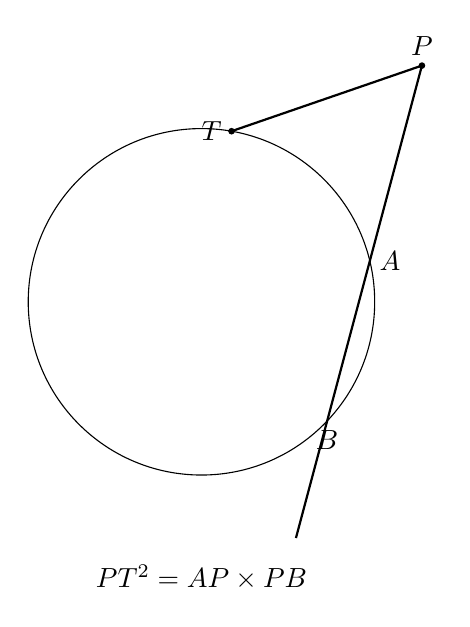
\begin{tikzpicture}[scale=1]
  \def\R{2.2}
  \coordinate (O) at (0,0);
  \draw (O) circle (\R);

  \coordinate (P) at (2.8, 3.0);

  % Tangent point
  \coordinate (T) at (80:\R);

  % Tangent line segment PT
  \draw[thick] (P) -- (T);

  % Secant through circle
  \coordinate (Q) at (1.2,-3.0);
  \path[name path=sec] (P) -- (Q);
  \path[name path=circle] (O) circle (\R);
  \path[name intersections={of=sec and circle, by={A,B}}];

  \draw[thick] (P) -- (Q);

  \fill (P) circle(1.2pt) node[above] {$P$};
  \fill (T) circle(1.2pt) node[left] {$T$};
  \node[right] at (A) {$A$};
  \node[below] at (B) {$B$};

  \node at (0,-3.5) {$PT^2 = AP\times PB$};
\end{tikzpicture}
\end{center}

\section*{Supplementary theorems}

\theoremblock{S1. Touching circles share a common tangent at the contact point}{Two circles touch if they have a common tangent at the point of contact.}{tangent of touching circles}
\diagram
\begin{center}
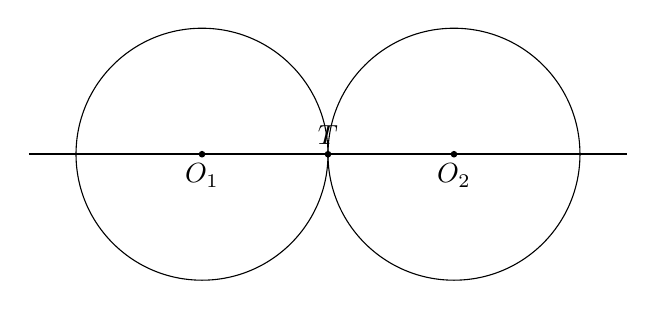
\begin{tikzpicture}[scale=1]
  \coordinate (O1) at (-1.6,0);
  \coordinate (O2) at ( 1.6,0);
  \def\R{1.6}

  \draw (O1) circle (\R);
  \draw (O2) circle (\R);

  \coordinate (T) at (0,0); % point of contact
  \draw[thick] (-3.8,0) -- (3.8,0); % common tangent (horizontal)

  \fill (O1) circle(1.2pt) node[below] {$O_1$};
  \fill (O2) circle(1.2pt) node[below] {$O_2$};
  \fill (T) circle(1.2pt) node[above] {$T$};
\end{tikzpicture}
\end{center}

\theoremblock{S2. Converse of ``angles in the same segment''}{If an interval subtends equal angles at two points on the same side of it then the endpoints of the interval and the four points are concyclic.}{converse of angles in the same segment}
\diagram
\begin{center}
\begin{tikzpicture}[scale=1]
  \coordinate (A) at (-2.2,-1.2);
  \coordinate (B) at ( 2.2,-1.2);
  \coordinate (C) at (-0.4, 1.8);
  \coordinate (D) at ( 1.2, 1.2);

  % Draw the (implied) circumcircle through A,B,C,D (using three points to define it)
  % Compute circumcenter of triangle A,B,C:
  \coordinate (Mab) at ($(A)!0.5!(B)$);
  \coordinate (Mac) at ($(A)!0.5!(C)$);
  \path[name path=pab] (Mab) -- ($(Mab)+(0,4)$);
  \path[name path=pac] (Mac) -- ($(Mac)+(-4,0)$);
  \path[name intersections={of=pab and pac, by=O}];

  \node[draw, circle through={(A)}] at (O) {};

  \draw[thick] (A) -- (B);
  \draw[thick] (A) -- (C) -- (B);
  \draw[thick] (A) -- (D) -- (B);

  \pic[draw, "$\theta$", angle radius=7mm] {angle = A--C--B};
  \pic[draw, "$\theta$", angle radius=7mm] {angle = A--D--B};

  \fill (A) circle(1.2pt) node[below left] {$A$};
  \fill (B) circle(1.2pt) node[below right] {$B$};
  \fill (C) circle(1.2pt) node[above left] {$C$};
  \fill (D) circle(1.2pt) node[above right] {$D$};
\end{tikzpicture}
\end{center}

\bigskip
\noindent\textbf{AAMT --- TOP DRAWER TEACHERS}\par
\noindent\textcopyright\ 2013 Education Services Australia Ltd, except where indicated otherwise.
This document may be used, reproduced, published, communicated and adapted free of charge
for non-commercial educational purposes provided all acknowledgements associated with the
material are retained.

\end{document}
